\cleardoublepage

\chapter{Resultados y conclusiones}
\label{makereference6}

%TODO EXPLICAR RESULTADOS Y CONCLUSIONES
%TODO AÑADIR FOTOS

\section{Calidad del código}
\label{makereference6.3}

\begin{figure}[htb]
	Una vez acabado el código del proyecto, decidimos certificar su calidad mediante \textbf{codacy}.
	\textbf{Codacy} es una herramienta que proporciona nuestro controlador de versiones \textbf{GitHub}. Sencillamente revisa todas y cada una de las líneas del código, para hacerlo más sencillo, escalable y seguro. Genera un informe con los errores y te dice qué grado de calidad tiene, siendo A el más alto. (\cite{ARP:Codacy:2017})
	
	\begin{center}
		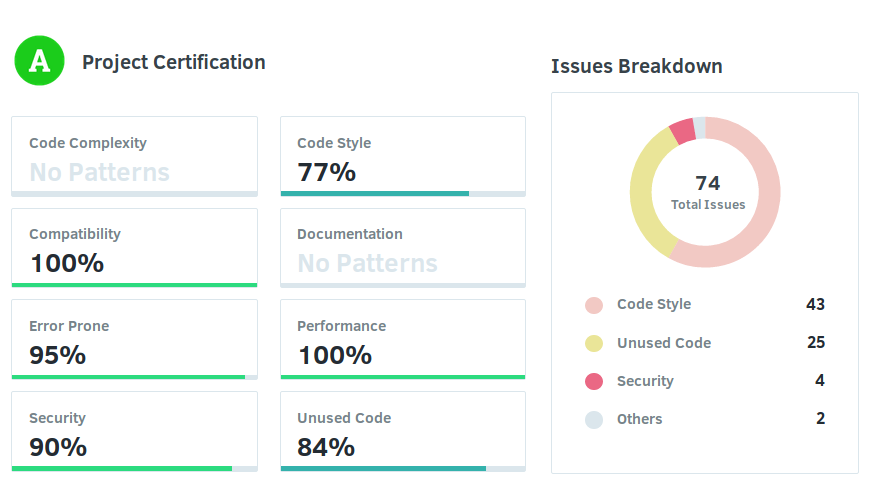
\includegraphics[height=3.5in]{figures/codacy.png}
		\caption{Informe de nuestro proyecto [Fuente: \href{https://www.codacy.com}{Codacy}]}
	\end{center}
	
	\label{codacy}
\end{figure}